% #############################################################################
% This is Chapter 5
% !TEX root = ../main.tex
% #############################################################################
% Change the Name of the Chapter i the following line
\fancychapter{Exploring Parameter-Efficient Strategies in Transfer Learning for Child-Focused ASR Systems}
\label{chap:5}
\cleardoublepage

\section{Introduction}
The use of increasingly larger models coupled with the abundance of massive datasets is driving rapid advancements in many domains of machine learning, encompassing NLP \cite{brown2020language} and computer vision \cite{ramesh2021zero}. In the context of ASR, this trend of scalling up models is exemplified by state-of-the-art models such as Whisper \cite{radford2023robust} and HuBert \cite{hsu2021hubert}, where the number of parameters can exceeds 1 billion. Research has underscored the interconnected nature of the training dataset size and the number of model parameters, identifying them as mutual bottlenecks that influence the performances of machine learning models. This observation accentuates the significance of scaling these two dimensions in tandem for the development of more robust and effective ASR models \cite{Kaplan2020ScalingLF}. Typically, to scalling up the model size a combination of an increased number of layers and an expansion of the model's hidden dimensions is used \cite{zheng22d_interspeech}.

However, the challenge arises when only a limited amount of data is available, making it challenging to train these large models from scratch, as highlighted by recent studies \cite{sri_end2end, gelin2021endtoend}. Hence, as discussed in the preceding chapter, transfer learning emerges as a well-established and effective paradigm to tackle to problematic of limited dataset. Nevertheless, despite its efficacy, we emphasised certain limitations that may potentially impede the performance of fine-tuning. Specifically, attempting to fine-tune these large models using a downstream dataset limited in size can be challenging. Indeed, in addition to be an expensive process, using small amount of data on such big model could potentially result in overfitting. This issue necessitates careful consideration, particularly in light of the recent evolution towards ever-growing pre-trained model sizes. Additionally, even following last chapter highlights where only specific parts of the model were fine-tuned, the different part of the model could be intricately linked to the overall model size. For example, FFN modules usually represent substantial portion, around 70\% of the total number of parameters. This insight underscores the persistence of the challenge associated with model size, even when fine-tuning only specific components. Finally, TL on large amount of parameters is memory-storage-inefficient, especially when there is a need to store a replicas of the billion of parameters models for many different small tasks.

Consequently, there is a growing need for more parameter-efficient transfer learning (PETL) as lightweight alternatives.
 %The use of increasingly bigger models in conjunction with the availability of massive datasets is driving rapid advancements across various domains of machine learning, including NLP and computer vision. In the context of ASR, this scaling up evolution is illustrated by state-of-the-art models such as Whisper and HuBert, where the number of parameters surpass 1 billion. Some research underscored the interconnected nature of the size of the training dataset and the number of parameters in model, as they both act as mutual bottlenecks in the pursuit of enhancing machine learning models. This critical observation highlight the importance of scaling these two dimensions in tandem for the development of better ASR models. Typically, the augmentation of the model's size results from a combination of an increased number of layers and an expansion of the model's hidden dimensions.
%However, when only limited amount of data is available it can be challenging to train these model from sratch \cite{sri_end2end,gelin2021endtoend}. Therefore, as discussed in the previous chapter, transfer learning emerges as a well-established and effective paradigm in this comtext. Nevertheless, despite its effectiveness, we underscored certain limitations that may potentially impede the efficacy of fine-tuning. Notably, challenges arise when fine-tuning large models using a downstream dataset limited in size. This is a crucial issue that requires careful consideration, particularly in light of the recent evolution of ever-growing size of pre-trained model. In addition, the process of fine-tuning specific parts of the model, such as the FFN modules for the Transformer, is intricately linked to the model size, as FFN modules often represents $\frac{2}{3}$ of the total amount of parameters.There is, then, a need for more parameters efficent approaches. Furthermore, TL from the large amount of parameters is storage-inefficient, especially when fine-tuning a model of billion of parameters for a lot of different small tasks. 
%In this context, the research community has introduced several parameter-efficient transfer learning (PETL) as a lightweight alternatives.
 Among the approaches introduced by the research community, residual Adapter modules stand out as the most popular and promising \cite{houlsby, pfeiffer}. Specifically tailored for Transformer-based systems, Adapters integrate a compact set of additional layers into a pre-trained source model. This design enables Adapters to enhance computational efficiency, resulting in faster training and addressing the challenge of catastrophic forgetting. Diverging from conventional transfer learning methods, where the source pre-trained model's weights are entirely replaced, Adapter-transfer maintains the integrity of the backbone model. Therefore, when the Adapter modules are removed, the initial pre-trained model remains unchanged. This preservation of the backbone model is a crucial advantage  as it offer increased flexibility. Furthermore, owing to their limited number of trainable parameters, Adapters demonstrate a decreased susceptibility to overfitting, thereby contributing to improved generalisation performance.


 In this chapter, our exploration is motivated by the promising characteristics of Adapters, and we will investigate their application in the specific context of children's ASR. The study will encompass the examination of diverse Adapter configurations within both Transformer and Conformer architectures. Additionally, a novel proposition involves the introduction of a speaker-group-based adapter using unsupervised cluster over speaker-embedddings.
The primary objective of this chapter is to address the overarching research question: \textit{Is it possible to develop an parameter-efficient automatic speech recognition model for children?} The investigation aims to unveil the potential for creating a model that optimally balances parameter efficiency and recognition accuracy. 
%In this context, the research community has introduced several parameter-efficient transfer learning (PETL) as a lightweight alternative.  Among these differents approaches, residual Adapter modules represents the most popular and promising PETL. Specifically designed for Transformer-based systems, Adapters integrate a compact set of additional layers into a pre-trained source model \cite{houlsby, pfeiffer}. This design allows Adapters to enhance computational efficiency, facilitating faster training and mitigating the issue of catastrophic forgetting.

%In contrast to conventional transfer learning approaches, where the source model's weights are entirely replaced, adapter transfer preserves the backbone model. Even when the adapter layers are removed, the underlying model remains unchanged. This retention of the backbone model provides a valuable advantage, allowing for greater flexibility and adaptability. Moreover, due to their limited number of trainable parameters, adapters exhibit a reduced susceptibility to overfitting, contributing to improved generalisation performances. Motivated by this, we will investigate ther use of ADapter in the context of children's ASR in this chapter. Different configuration in the context of both Transfromer and Conformer will be presented. Then, as comparaison to Adapter we will investigate the use of other PETL in the context of children ASR. Finally, we will propose a new type of Adapter, the shared-Adapters, that use the overparameterisation present in Transformer-based model to reduce the number of parameters.



%In response to these challenges, the research community has introduced lightweight alternatives for fine-tuning, known as parameter-efficient transfer learning (PETL).Residual adapter modules represents an popular PETL approach, especially to address the problems in traditional transfer learning. Adapters, specifically designed for Transformer-based systems integrate a compact set of additional layers into a pre-trained source model \cite{houlsby, pfeiffer}. These Adapters typically provide enhanced computational efficiency, resulting in faster training and mitigating the problem of catastrophic forgetting. In contrast to conventional transfer learning, where the source model's weights are completely replaced, adapter transfer preserves the backbone model, leaving it unchanged even when the adapter layers are removed. Additionally, due to their limited number of trainable parameters, adapters tend to be less prone to over-fitting.
%As presented in the previous chapter, transfer learning, despite beeing a well-established and well-performing paradigm has some limitations. Especially when it comes to fine-tuning large models with a limited-size downstream dataset. However, the availability of massive datasets and the development of ever-growing size model allowed rapid progress in many field of machine learning, from NLP, computer vision and ASR. Examples of such models like Whisper and HuBert can go up to more than 1 billion parameters. In addition, the size of the training dataset and the number of model parameters are mutual bottlenecks and must be scaled in tandem, which is a important information for the development of better ASR models.  Usually, the models size are increase by a conjounction of increased number of layer, model's dimension.  As a consequence, fine-tuning part of the model, such as the FFN layers only, can also drasticly increase. 
%More recently, advances on self-supervised learning (SSL)  focused on training models to extract representations from large volumes of unsupervised data. Subsequently, the entire network undergoes fine-tuning to use the extracted representations effectively in supervised tasks. Notably, these advances have led to significant improvements in child speech recognition\cite{9847929,fan2022draft}. However, fine-tuning the entire network in this way can lead to significant computational costs, including long training times and substantial storage requirements. Moreover, SSL is vulnerable to domain shift, when the data domain used for fine-tuning differs from the initial pre-training domain. Although SSL yields improved performances with extensive unlabeled data during pre-training, recent research suggests that even greater improvements can be achieved by including target domain data during the pre-training phase \cite{hwang2022large}.
%However, larger models require more data for effective fine-tuning to prevent over-fitting. 
%Residual adapter modules offer an alternative approach to address traditional transfer learning limitations in the context of automatic children's speech recognition of large ASR models. Adapters, specifically designed for Transformer-based systems integrate a compact set of additional layers into a pre-trained source model \cite{houlsby, pfeiffer}. These adapters typically provide enhanced computational efficiency, resulting in faster training and mitigating the problem of catastrophic forgetting. In contrast to conventional transfer learning, where the source model's weights are completely replaced, adapter transfer preserves the backbone model, leaving it unchanged even when the adapter layers are removed. Additionally, due to their limited number of trainable parameters, adapters tend to be less prone to over-fitting.

%In this chapter, we extend research presented in \cite{chen2023efficient} and \cite{10095837} by conducting a comprehensive evaluation of various adapter  and other PETL configurations specifically designed for Conformer models in the domain of children's speech recognition. Furthermore, we introduce a two adapter configurations, the Two Serial Adapter (TSA) and Shared-Adapter. We also considering the potential benefits of age-dependent acoustic models, and given the strong correlation between children's age and acoustic variability \cite{gale2019improving, shivakumar2020transfer}, we propose a novel cluster-based strategy for training adapters.

\section{Adapter tuning}

\begin{figure*}[t]
    \begin{center}
    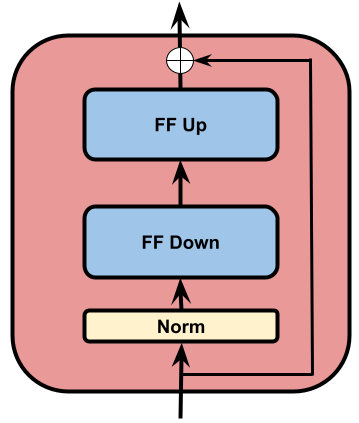
\includegraphics[scale=0.3]{imgs/Adapter_alone.png}
    \caption{Residual Adapter architecture}
    \label{fig:Adapter_architecture}
    \end{center}
    \end{figure*}


Adapters were initially introduced in the NLP field to efficiently adapt large models, such as Transformers, using minimal amount of parameters for text classification \cite{houlsby}. As an alternative to full model fine-tuning, Adapter-transfer involves training an extra small number of task-specific parameters while keeping the original model frozen. This is done at each Transformer layer level by plugging them after the Multi-Head Attention (MHA) and Feedforward Neural Network (FFN) modules, a setup often referred to as the \textit{Houlsby} configuration. Subsequently, \cite{pfeiffer} demonstrated that Adapters placed only after the FFN modules were sufficient for achieving efficient performances, referred to as the \textit{Pfeiffer} configuration. Generally, Adapters employ a bottleneck architecture, consisting of a normalisation layer followed by a projection-down linear layer with a non-linear activation, and subsequently a projection-up linear layer. Finally, a residual connection is applied by summing the input of the Adapter with its output. The overall structure is illustrated in Figure \ref{fig:Adapter_architecture}. Research suggests that the hidden dimension, between the down and up projections, may not always benefit from a bottleneck structure, where $d_{hidden} < d_{model}$, and the optimal design may vary depending on the downstream task. In some tasks, an hidden dimension larger than the model size itself, in other words $d_{hidden} > d_{model}$, has been proven more effitive \cite{fan2022draft}.

Some of the main advantages of Adapters are their parameter efficiency and modularity. This efficiency is particularly interesting when working with large pre-trained models, while the modularity is valuable when a large number of tasks need to be trained.
Mathematically, the structure of an Adapter can be expressed as follows:
%Adapters were first introduced in the natural language processing field to efficiently adapt large models like Transformers for text classification \cite{houlsby}. They are a simple alternative to full model fine-tuning, adding a small number of parameters at each transformer layer, generally after the feed-forward layer. Adapters use a bottleneck architecture (projection-down followed by projection-up) and have benefits such as parameter efficiency, faster training, and modularity compared to full fine-tuning. Adapter can be expressed as follows:
\begin{equation}
    adapter(x) = x + (W_{up}(f(W_{down}g(x)+b_{down})))+ b_{up})
\end{equation}
Where $W_{down}$ and $W_{up}$ denote the weights of the projection-down and projection-up linear layers, and $b_{down}$ and $b_{up}$ represent the corresponding biases. The function $f(\cdot)$ is a non-linear activation, while $g(\cdot)$ a layer normalisation or identity function. Finally, $x$ corresponds the input given to the Adapter.

In terms of computation, Adapters offer the advantage of faster training, given that they update fewer parameters compared to fully fine-tuning models. However, there might be a slight processing delay during inference due to the addition of extra parameters introduced by the Adapters, this difference is generally minimal and can be well-managed \cite{ruckle2020adapterdrop}.

% Adapter ASR
Adapter-transfer has gained increased attention in the context of ASR tasks \cite{cappellazzo2023parameter,chen2023efficient,10095837}, particularly owing to its modular nature, which has proven advantageous in the context of multi-lingual ASR \cite{kannan2019large, hou2021exploiting, kulkarni2023adapting}. In these studies, distinct Adapters were trained for each language, contributing to enhanced performance compared to a monolingual model and mitigating certain challenges associated with transfer learning, such as overfitting. This modular approach provides a tailored solution, as each Adapter designed for a specific language can effectively capture the diverse acoustic characteristics unique to that language.



In addition, researchers have explored the use of Adapters in the context of SSL. In SSL, larger model are typically employed to capture a wide range of information from speech for application in a broad spectrum of tasks \cite{thomas2022efficient, fan2022draft}. However, the computational cost and scalability to multiple tasks can pose a challenge. Notably, once the model is fine-tuned for a specific task, the entire model is fixed for that task, and re-loading and re-training the base model are necessary for transferring to a different task. Therefore, the use of Adapters has proven effective in addressing these challenges by providing a modular and parameter-efficient task-specific adaptation.


Additionally, the effectiveness of Adapters has been demonstrated in addressing challenges related to low-resource and atypical speech recognition scenarios \cite{tomanek2021residual}

Finally, the effectiveness of Adapters has also been demonstrated in addressing challenges related to low-resource and atypical speech recognition scenarios \cite{tomanek2021residual}. In such scenarios, similarly to children's speech, there is limited availability of labeled data and atypical speech characteristics. As a result, Adapters provide a valuable solution by efficiently adapting large pre-trained models to these challenging tasks. 

% Adapter children
However, the application of Adapters in the context of children's ASR has received limited attention, with only one notable study by \cite{fan2022draft}. In this study, the authors proposed integrating and training Adapters within SSL models, followed by fine-tuning the entire model, including the adapter weights, for better modeling of children's speech. This represents a pioneering effort to leverage Adapters for adapting large-scale models to the unique characteristics of children's speech.
%Finally, Adapters in the context of children's ASR have received limited attention, with only one notable study by \cite{fan2022draft}, who proposed integrating and train Adapters into SSL models and subsequently fine-tuning the entire model, including the adapter weights for better modelling of children's speech. 
%In contrast, our primary objective is to update only the adapter weights during supervised training, maintaining the parameter efficiency and modularity of adapters, without relying on semi-supervised pre-training.

\section{Investigating ASR for Child Speech with Adapters}


\begin{figure*}[t]
    \begin{center}
    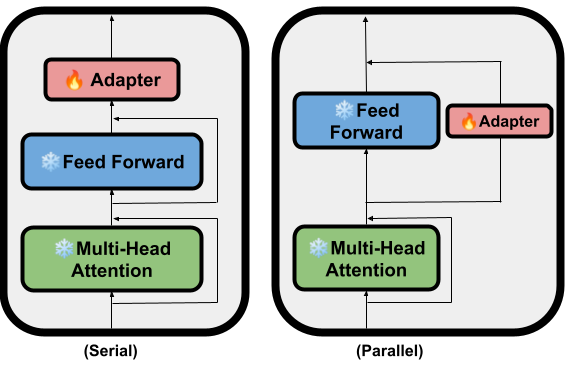
\includegraphics[scale=0.27]{imgs/Adapter_Transformer.png}
    \caption{Transformer block with various residual adapter configurations. Normalisation layers are not display in this figure}
    \label{fig:transformer_config}
    \end{center}
\end{figure*}
\begin{figure*}[t]
    \begin{center}
    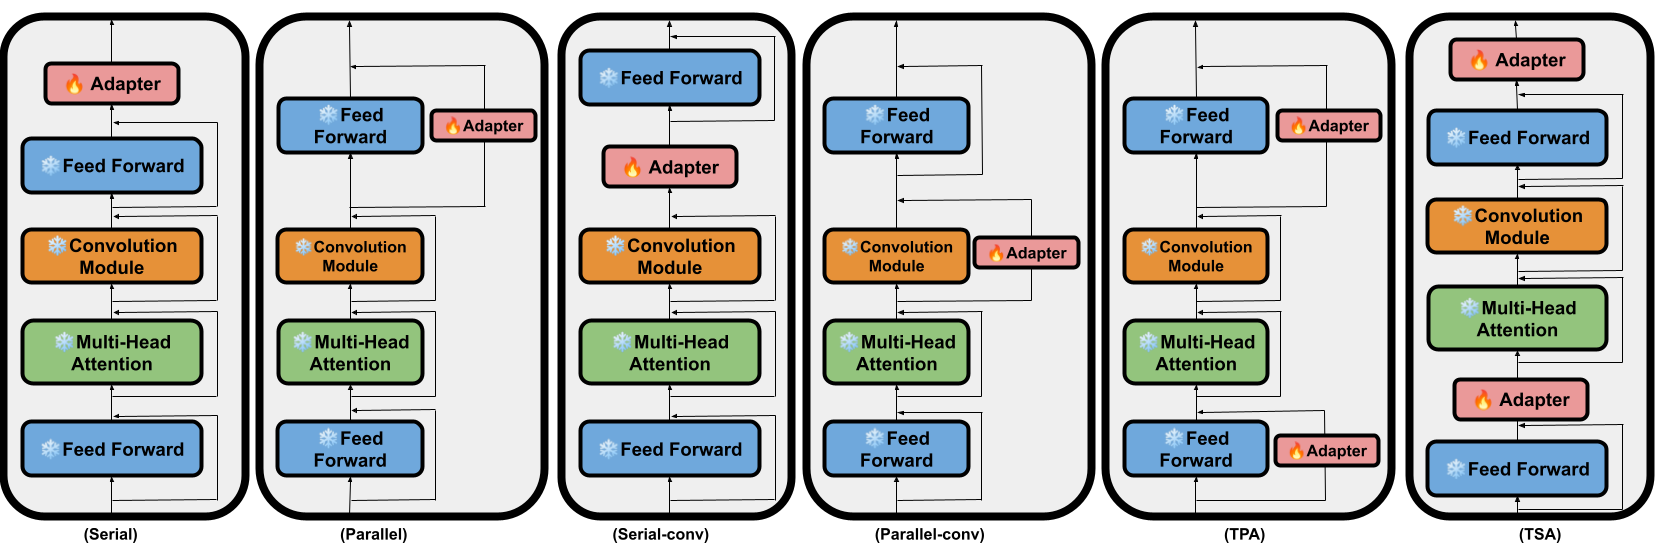
\includegraphics[scale=0.27]{imgs/Adapter_conformer.png}
    \caption{Conformer block with various residual adapter configurations. Normalisation layers are not display in this figure}
    \label{fig:conformer_config}
    \end{center}
\end{figure*}

In this section, we delve into the application of Adapter-transfer as PETL for both Transformer and Conformer architectures in the domain of children's ASR. Building upon our findings from the previous chapter, where we identified the FFN modules as the most relevant component to fine-tuning in a Transformer-based model, we opt to leverage Adapters for modifying the output of these FFN modules. Additionally, considering our results that underscore the significance of fine-tuning the Encoder, our primary emphasis will be on investigating the implementation of Adapters within the Encoder. Specifically, for the Transformer architecture, we investigate two integration methods: parallel and serial placement with the FFN component. Such configurations were used in prior work \cite{he2021towards} and are depicted in Figure \ref{fig:transformer_config}.

In the case of the Conformer architecture, we explore six distinct Adapter configurations, as illustrated in Figure \ref{fig:conformer_config}. The initial two configurations mirror our Transformer investigation, involving both parallel and serial placements, either after or in parallel with the second FFN layer \cite{chen2023efficient}. Additionally, we assess a configuration that introduces an Adapter following the convolution module, denoted as the "serial-conv" setup used in \cite{10095837}. Notably, although the FFN component has been identified as the most crucial for fine-tuning, promising results have also been observed by fine-tuning the convolution modules \cite{chen2023efficient}. Furthermore, \cite{chen2023efficient} introduces two variants of the parallel setup: "parallel-conv," where the Adapter operates in parallel with the convolution module, and "TPA," which deploys two adapters in parallel with both FFN modules in the Conformer layer. This comprehensive exploration of Adapter configurations within both architectures aims to discern the most effective adaptation strategies for children's speech in the context of ASR. 


In the case of serial configurations, the integration of adapter information is performed with the preceding component denoted as $P$. The specific component $P$ varies depending on the configuration and can be either FFN or convolution modules. This integration is realised through the following process:

\begin{equation}
    output =  Adapter(P(x))
\end{equation}

where $x$ represents the input of component $P$.

For parallel configurations, the integration process varies slightly. In this scenario, the adapter's output is combined with the output of component $P$ as follows:

\begin{equation}
    output = x + 0.5 \cdot P(x) + (Adapter(x) - x)
\end{equation}

where $x$ is the input of component $P$.

To comprehensively explore all feasible configurations, we introduce two novel setups. The first one is referred to as "Two Serial Adapters" or "TSA," where two Adapters are sequentially positioned after each FFN component in all layers. The second configuration combines TPA and TSA, resulting in the integration of four Adapter modules both in parallel and serially at the two FFN modules level. 
%To fully explore all feasible configurations, we introduce two novel configurations respectively called Two Serial Adapters or "TSA" where two Adapters are positioned sequentially after each FFN component in all layers. The second configuration is the combination of the TPA and TSA where four Adapters modules are integrated both in parallel and serial at the two FFN modules level.

Moreover, we consider three distinct configurations where Adapters are placed in the Decoder. It is important to note that in the Conformer architecture, the decoder is a regular Transformer. Therefore, we evaluate the "Serial" and "Parallel" setups. Subsequently, we investigate the combination of the most effective encoder Adapter configuration with both Decoder configurations. To the best of our knowledge, there is no prior research that formally investigates the influence of Adapters within an ASR decoder. 
%In the case of serial configurations, we integrate the adapter information with the preceding component denoted as $P$. The specific component $P$ varies depending on the configuration and can be either the FFN or the convolution modules. This integration is accomplished through the following process:
%\begin{equation}
%    output =  Adapter(P(x))
%\end{equation}
%In the parallel configurations, the integration process differs slightly. Here, we combine the adapter's output with the output of component $P$ as follows:
%\begin{equation}
%    output = x + 0.5 * P(x) + (Adapter(x) - x)
%\end{equation}
%where $x$ is the input of the component $P$. In order to comprehensively explore all feasible configurations, we introduce a novel one called ``TSA,'' which stands for Two Serial Adapters. In this configuration, one Adapter is positioned sequentially after each FFN component.

%Additionally, for a comprehensive assessment of Adapter behaviour, we consider three distinct configurations where Adapters are placed in the Decoder. Note that in the Conformer architecture, the decoder is a regular Transformer. Therefore, we initially evaluate the ``Serial''and ``Parallel''setups. Subsequently, we investigate the combination of the most effective encoder Adapter configuration with both Decoder configurations. To the best of our knowledge, there is no prior research that formally investigates the influence of Adapters within an ASR decoder.%

% Finally, we explore the use of unsupervised clustering of utterances, motivated by the strong correlation between children's speech variability and age. Our aim is to create clusters of utterances that exhibit similar acoustic characteristics. This process employs a k-means clustering algorithm on the x-vector representation \cite{snyder2018x} of each training utterance. The primary objective is to investigate whether Adapters trained on comparable speech characteristics yield improvements over a general Adapter on the entire training set. To evaluate this approach, we use this clustering in the test set, where test utterances are decoded with their respective cluster Adapters.

Finally, motivated by the observed strong correlation between children's speech variability and age, we explore the possibility of training specialised Adapters. However, considering the high inter-speaker variabilities in children's speech, using age directly may not effectively capture children with similar acoustic characteristics. Additionally, in many children's speech datasets, precise age information is often not provided. To address this, we partition the training dataset into groups of speakers with similar acoustic characteristics based on unsupervised clustering.
In practice, we apply a k-means clustering algorithm on the x-vector representation \cite{snyder2018x} of all training utterances. Subsequently, distinct Adapters are trained for each speaker cluster separately. During the testing phase, the closest clusters of group of speaker is determined for each test utterance, and the corresponding Adapters specific to that group are employed for decoding.

%Finally, motivated by the strong correlation between children's speech variability and age, we investigate the possibility of training specialized Adapters for groups of speakers exhibiting similar acoustic characteristics based on unsupervised clustering. In practice, we apply a k-means clustering algorithm on the x-vector representation \cite{snyder2018x} of each training utterance. Then, a different adapter model is trained for each  speaker cluster. During test, the closest speaker cluster is found for each test utterance and the corresponding Adapter weights are used for decoding.
The primary objective of these experiments is to investigate whether Adapters trained on comparable speech characteristics yield improvements over a general Adapter on the entire training set. Indeed,
%\subsection{Relation to prior work}
%\label{sec:prior}
% No work fully compared Adapter vs Conformer in Children speech
children's speech is inherently atypical and displays a significant degree of variability, making it imperative to assess the efficacy of existing methods. In prior work, different configurations were employed resulting in a lack of standardised evaluation.

\section{Implementation details}

All experiments were performed using the SpeechBrain toolkit \cite{speechbrain}. We used  12 Transformer or Conformer layers for the encoder, for the Transformer and Conformer model respectively, and 6 Transformer layers for the decoder, all with dimensions 512. These models have been pre-trained using the LibriSpeech dataset \cite{librispeech} and are publicly available\footnote{https://huggingface.co/speechbrain/asr-transformer-transformerlm-librispeech} \footnote{https://huggingface.co/speechbrain/asr-conformer-transformerlm-librispeech}. Furthermore, for all of our experiments, we used the same Transformer language model, trained on 10 million words 
%CAMERA-READY (Add Information about the Language model training)
on the LibriSpeech transcriptions.
The adapter architecture consists of a  first linear layer projection to dimension 512 with a ReLu activation, followed by another linear layer projection to dimension 512 with a residual connection of the adapter input. For all Adapters, in the initialisation process, we set $W_{down}$ to all zeros, and $W_{up}$, $b_{down}$, $b_{up}$ are initialised using Xavier initialisation \cite{glorot2010understanding}.


The use of a hidden-dimension size equal to the model size (instead of a bottleneck) was motivated by previous research exploring hidden-dimension size, that consistently demonstrated that larger dimensions tend to yield improved performance scores \cite{chen2023efficient}.
All models were trained for 30 epochs, with a learning rate of $8\cdot10^{-4}$ for Adapters experiments and of $8\cdot10^{-5}$ for fine-tuning the entire model.
For the clustering experiments, we use the k-means clustering algorithm on the speaker-embedding of each utterance. The speaker embeddings were extracted using a publicly pre-trained ECAPA-TDNN model, trained on adult speech\footnote{https://huggingface.co/speechbrain/spkrec-ecapa-voxceleb}.

\section{Results}
\label{sec:results}

\subsection{Configurations}
\begin{table}[t]
\caption{Results of the different Adapters configurations in both Transformer and Conformer.}
\begin{center}    
\begin{tabular}{ccc}
\hline
 Method & WER $\downarrow$     & Trained params    \\ \hline \hline
\multicolumn{3}{c}{Transformer} \\ \hline
\multicolumn{1}{l}{\textit{Frozen}} & 25.04\%   & - \\
\multicolumn{1}{l}{\textit{Full fine-tuning}} & 12.99\% & 71.5M \\ \hline
\multicolumn{1}{l}{Serial}  &   12.78\% & 6.3M  \\ 
\multicolumn{1}{l}{Parallel}  &     \textbf{12.62\%} & 6.3M  \\ \hline\hline
\multicolumn{3}{c}{Conformer} \\ \hline
\multicolumn{1}{l}{\textit{Frozen}} & 21.75\%   & - \\ 
\multicolumn{1}{l}{\textit{Full fine-tuning}} & 12.28\% & 109.1M \\ \hline
\multicolumn{1}{l}{Serial}  &   11.76\% & 6.3M  \\ %11.84 
\multicolumn{1}{l}{Serial-Conv} & 11.78\%     & 6.3M  \\
\multicolumn{1}{l}{Parallel}    & 11.72\% & 6.3M  \\ % 11.88 
\multicolumn{1}{l}{Parallel-conv} & 11.79\%      & 6.3M  \\ %\hline
\multicolumn{1}{l}{TPA} & \textbf{11.58\%}     & 12.6M  \\ %11.85
\multicolumn{1}{l}{TSA} & 11.75\%     & 12.6M  \\ \hline %11.72
\multicolumn{1}{l}{Serial (Decoder)} & 18.09\%     & 3.2M  \\ 
\multicolumn{1}{l}{Parallel (Decoder)} &17.76\%     & 3.2M  \\ \hline
%\multicolumn{1}{l}{TPA + Serial (Decoder)} & 00.00(T)\%     & 15.8M  \\
%\multicolumn{1}{l}{TPA + Serial (Decoder)} & 11.68\%     & 15.8M  \\ 
\multicolumn{1}{l}{TPA + Parallel (Decoder)} & \textbf{11.47\%}     & 15.8M  \\ \hline

\end{tabular}
\end{center}

\label{tab:res}
\end{table}

In this section, we present a comprehensive evaluation of Adapter configurations applied to both Transformer and Conformer models, assessing their performance based on Word Error Rate (WER), as presented in Table \ref{tab:res}.  First, we assess 
%CAMERA-READY ( remove this to make more clear that frozen is no-finetune and without adapters)
%Adapter configurations in 
the Transformer model when no fine-tuning was applied (\textit{Frozen}), resulting in a WER of 25.04\%. Conversely, \textit{Full Fine-Tuning} involved complete fine-tuning of the entire model,
%CAMERA-READY (Make more clear that this is our baseline)
working as our baseline system
, reducing the WER significantly to 12.99\%, at the expense of 71.5 million trainable parameters.
Turning to the Adapter setups, we investigate the ``Serial'' and ``Parallel'' configurations, both equipped with 6.3 million trainable parameters. The ``Parallel''emerged as the best configuration, achieving the lowest WER of 12.62\% compared to 12.78\% for the ``Serial``. These results underscore the effectiveness of Adapter configurations within the Transformer architecture, as they both perform slightly better than the full-finetuning.

Next, we investigated the Conformer model, we once again explored \textit{Frozen} and \textit{Full Fine-Tuning}. In \textit{Frozen} the pre-trained model remained untouched, yielding a WER of 21.75\%. The Full fine-tuning, in a similar way as the Transformer, led to enhanced performance, reducing the WER to 12.28\% with a total of 109.1 million trainable parameters. We can observe that given the same pre-training dataset, the Conformer architecture outperforms the regular Transformers. Within the set of adapter configurations, ``Serial'' achieved a WER of 11.76\%, while ``Parallel'' demonstrated slightly better performance with a WER of 11.72\%. These results indicated that ``Parallel''Adapters were more effective in improving WER in the Conformer model. When Adapters are placed after the convolution layer, with the ``Serial-conv'' and ``Parallel-conv'' configuration, both slightly under-perform compared to Adapters placed after the second FFN component with respective scores of 11.78\% and 11.79\%. Finally, we evaluated the ``TPA''and ``TSA''configurations. The ``TPA''configuration emerged as the most promising, with a very remarkable WER of 11.58\% using 12.6 million trainable parameters, while ``TSA''achieved a WER of 11.75\%, which is slightly under-performing compared to the ``TPA''configuration.

In addition, we evaluated the use of  Adapters in the decoder. As the decoder of the Conformer architecture is a regular Transformer, we only evaluate the ``Serial''and ``Parallel'' setup, which respectively reached 18.09\%  and 17.76\% WER with 3.2 million parameters. Results showed that Adapters are more relevant when plugged into the encoder. It confirms that acoustic variability plays a critical role in the degradation of children's ASR performance. Finally, combining ``TPA''in the encoder layers with ``Parallel''Adapters in the decoder outperforms Adapters in the encoder only, with 11.47\% WER. Consequently, this configuration stands as the most effective model. 

%statistical tests
We performed statistical tests (Matched Pairs Sentence-Segment Word Error) across all Adapter setups in comparison to the full fine-tuning configuration using SCTK, the NIST Scoring Toolkit \footnote{https://github.com/usnistgov/SCTK/tree/master}. 
The results reveal that, in all scenarios, the \textit{p}-value is less than or equal to 0.001. This observation denotes statistical significance, indicating evidence against the null hypothesis. 

These results collectively illustrate the versatility and effectiveness of different Adapter configurations within the Transformer and  Conformer model for the children's ASR task. ``TPA''Adapters in the Encoder combined with ``Parallel''Adapters in the Decoder showcased outstanding performance, highlighting their potential as a fine-tuning replacement in large model children ASR scenarios.

\subsection{Effect of the Adapter hidden dimension}
\begin{figure}
    \begin{center}
    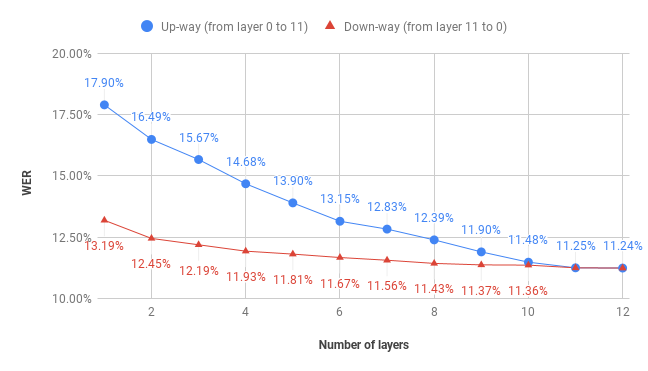
\includegraphics[scale=0.5]{imgs/layerTL.png}
    \caption{Experimental Adapter transfer using different hidden dimension size within the Conformer architecture }
    \label{fig:HiddenDim}    
\end{center}
    
\end{figure}

In this section, our aim is to investigate the impact of varying the hidden dimension $d_{hidden}$ on the performance of the model. While our previous experiments used a context hidden dimension equal to that of the model, here 512, we will explore different hidden dimension values within the Conformer architecture, specifically employing the TPA in the Encoder-only configuration. This investigation evaluate how variations in the hidden dimension may influence the performance of the Adapter transfer, providing valuable insights into the parameter tuning process for Adapter modules.

In Figure \ref{fig:HiddenDim}, the WER performances of the Adapter transfer are presented in relation to the hidden dimension size ($d_{hidden}$). Notably, a delicate balance is observed, emphasising the importance of choosing an optimal hidden dimension size. Configurations with dimensions that are either too small or too large result in a degradation of overall performance. The best-performing configuration aligns with the choices made in all previous experiments, with $d_{hidden} = d_{model} = 512$. This observation supports the hypothesis that the parallel Adapter functions as an extension of the key-value memory of the FFN. Opting for an extremely large hidden dimension makes training more complex due to the large amount of parameters, while an excessively small size drastically limits the potential information learned in the Adapters. 

\subsection{Unsupervised clustering for grouped-speaker Adapters}
\begin{table}[t]
\caption{Results of the clustering approach.}
\begin{center}    
\begin{tabular}{cc}
\hline
  \# of clusters & Average WER $\downarrow$    \\ \hline
\multicolumn{1}{c}{1} & 11.58\%  \\% OR 11.70%  If we consider 40 epochs instead of 30 here
\multicolumn{1}{c}{2} & \textbf{11.50\%}  \\
\multicolumn{1}{c}{3} & 11.57\%  \\
\multicolumn{1}{c}{4} & 11.51\%  \\ \hline 

\end{tabular}
\end{center}

\label{tab:res_clusters}
\end{table}

In this section, we present the outcomes of our clustering approach, as summarised in Table \ref{tab:res_clusters}. The investigation focused on the influence of varying the number of cluster on the ASR performance, ranging from 1 to 4 clusters, using the ``TPA" configuration in an encoder-only setup. First, when the data remained unclustered (one cluster), the ASR system exhibited a 
WER of 11.58\%. Notably, the two-cluster configuration outperformed the other setups, achieving a superior performance with a WER of 11.50\%. This result suggests that partitioning the data into two distinct clusters allows the different Adapters to more effectively capture underlying patterns intricately linked to their respective clusters, consequently enhancing the recognition scores.
Furthermore, we explored the impact of increasing the number of clusters to three and four, revealing only marginal differences in performance. Specifically, the three-cluster configuration yielded a WER of 11.57\%, and the four-cluster configuration resulted in a WER of 11.51\%. These findings underscore the role of data clustering in children's ASR systems by grouping shared speaker characteristics in different clusters.

In summary, our investigation underscores the significance of data clustering in children's ASR systems. The optimal performance was achieved with a two-cluster configuration, suggesting that this approach enables the Adapters to capture cluster-specific patterns effectively. The marginal differences observed with three and four clusters highlight a potential saturation point where further partitioning offers diminishing returns in terms of ASR performance improvement.

%In this section, we present the outcomes of our clustering approach, as summarised in Table \ref{tab:res_clusters}. We investigated the influence of varying cluster numbers on ASR performance, ranging from 1 to 4 clusters using the ``TPA''in the encoder-only configuration. Notably, when the data remained unclustered (one cluster), the ASR system exhibited a WER of 11.58\%. However, the two-cluster configuration surpassed the others, achieving a superior performance of 11.50\%. This result suggests that partitioning the data into two distinct clusters enables the Adapters to more effectively capture underlying patterns intricately linked to their respective clusters, consequently enhancing the recognition scores. Furthermore, we explored the impact of increasing the number of clusters to three and four, revealing only marginal differences in performance, with WERs of 11.57\% and 11.51\%, respectively. These findings underscore the role of data clustering in children's ASR systems.

\section{Summary and discussion}
% Summary
In this chapter, our exploration centered around investigating the viability of Adapter transfer in the context of children's ASR. We answer the following research question \textit{Is it possible to develop an parameter-efficient automatic speech recognition model for children?} by a positive answer. Our study demonstrated the efficacy of efficiently adapting the model using Adapter modules, showcasing improved WER performances compared to full-model fine-tuning, all while utilising only around 10\% of the parameters required in the traditional transfer learning configuration. Among the diverse configurations examined in this chapter, the Parallel Adapter and its extension, the TPA, emerged as the most effective choices for the Transformer and Conformer architectures, respectively. This parallel Adapter can be perceived as an extension of the key-value memory that represent the FFN modules, showcasing its potential for capturing essential children information in a more parameter-efficient manner.

Expanding upon our findings, we proposed to incorporate an unsupervised clustering on the speaker embeddings extracted the different utterances to the Adapter transfer procedure. This strategic separation aimed to facilitate the training of specific Adapters for each cluster, offering a more personalised adaptation without requiring detailed metadata about the speaker, such as their age. Our results demonstrated that leveraging these clusters could further enhance the overall performances, paving the way for the application of Adapters in personalised ASR systems.

% Discussion
% Mention that this open the way for other used, such as reducing the domain mismatch
The feasibility of Adapter transfer in the domain of children's speech opens up new avenues for advancing children's ASR. Our findings indicate that Adapters effectively bridge the gap between source and target domains, while preserving the pre-trained models and the knowledge it contains. This promising result paves the way for further research. In the upcoming chapter, we will explore the application of Adapters in the realm of TTS data augmentation. This extension of our research seeks to leverage the capabilities of Adapters for reducing the gap between real and synthetic children speech.
% Also mention that we will investigate other PETL approaches
In addition to presenting the Adapter module in this chapter, it is worth noting that a new variety of PETL approaches exist in the literature, showcasing their effectiveness in tasks beyond children's ASR such as NLP tasks. Our exploration will extend to these new existing PETL modules, assessing their applicability and performance in the context of children's ASR. Additionally, we will delve into the development of new PETL approaches, aiming to strike a balance between parameter efficiency and accuracy. 


